\documentclass{article}

\usepackage{tikz}
\usepackage{xcolor}
\usepackage{xltxtra}
\usepackage{listings}
\usepackage{hyperref}
\usepackage{tikz-3dplot}

\hypersetup{
    colorlinks=true,
    linkcolor=blue,
    filecolor=magenta,
    urlcolor=cyan,
    citecolor=blue,
    pdfpagemode=UseOutlines,
    pdfstartview={FitH},
    pdfdisplaydoctitle=true,
    unicode=true,
}

\definecolor{codegreen}{rgb}{0.3,0.6,0.3}
\definecolor{codegray}{rgb}{0.5,0.5,0.5}
\definecolor{codepurple}{rgb}{0.5,0,0.33}
\definecolor{backcolour}{rgb}{0.95,0.95,0.92}

\lstset{numberstyle=\tiny\color{codegray},
    stringstyle=\color{blue},
    basicstyle=\ttfamily\footnotesize,
    breakatwhitespace=false,
    breaklines=true,
    captionpos=b,
    keepspaces=true,
    numbers=left,
    numbersep=5pt,
    showspaces=false,
    showstringspaces=false,
    showtabs=false,
    tabsize=8,
    language=C,
    morekeywords={size_t, off_t, ssize_t, bool, true, false},
}

\lstset{
    emph=[1]{%
        for, while, do, if, else, switch, case, default, break, continue, return, typedef, struct, enum,
        union, typedef, sizeof, NULL, static, extern, const, volatile, register, inline, restrict,
        int, char, short, long, float, double, unsigned, signed, void, auto
    },
    emphstyle=[1]\color{codepurple}\bfseries,
}

\lstset{
    emph=[2]{%
        //, /*, */
    },
    emphstyle=[2]\itshape,
}

\lstset{
    numbers=right,
    numberstyle=\tiny\color{codegray},
}

\lstset{
    emph=[3]{%
        \documentclass, \usepackage, \title, \author, \date, \section, \subsection, \caption, \label,
        \ref, \eqref, \textbf, \emph, \textit, \texttt, \textcolor, \definecolor, \lstset, \emphstyle
    },
    emphstyle=[3]\color{blue},
}

\title{Ivenbox - Sistemas Embarcados}
\author{Henrique Brocco \and Lucas Diniz \and João Martins \and Pedro Igor}
\date{\today}

\begin{document}
\maketitle
\section{Visão Geral do Sistema}
Este projeto consiste em um sistema de monitoramento de condições ambientais dentro de um recipiente hermético que abriga alimentos. Através de um ESP32, o sistema monitora a temperatura e umidade dentro do recipiente e ativa uma ventoinha caso a temperatura exceda um valor definido. Além disso, o sistema também monitora se o recipiente está cheio através de um sensor infravermelho. Todas as informações são exibidas para o usuário através de um display LCD 16x2.
\section{Estrutura do projeto}
\tdplotsetmaincoords{60}{60}
  \begin{figure}[ht!]
    \centering
  \begin{tikzpicture}[
      scale=0.92,
      tdplot_main_coords,
      grid/.style={very thick,gray},
      axis/.style={->,gray,very thick},
      cube/.style={very thick},
      cube hidden/.style={very thick,dashed},
      curve/.style={dashed,thick}]

      \coordinate (O) at (0,0,0);

      \draw[axis] (0,0,0) -- (4,0,0) node[anchor=west]{$x$};
      \draw[axis] (0,0,0) -- (0,4,0) node[anchor=west]{$y$};
      \draw[axis] (0,0,0) -- (0,0,6) node[anchor=west]{$z$};

      \draw[cube] (0,0,0) -- (0,2,0) -- (2,2,0) -- (2,0,0) -- cycle;
      \draw[cube] (0,0,4) -- (0,2,4) -- (2,2,4) -- (2,0,4) -- cycle;


      \draw[cube hidden] (2,0.2,1.5) -- (2,1.8,1.5) -- (0.2,1.8,1.5) -- (0.2,0.2,1.5) -- cycle;
      \draw[cube hidden] (2,0.2,3.5) -- (2,1.8,3.5) -- (0.2,1.8,3.5) -- (0.2,0.2,3.5) -- cycle;

      \draw[cube] (2,0.3,0.4) -- (2,1.7,0.4) --
      (2,1.7,1.2) -- (2,0.3,1.2) -- cycle;

      \draw[cube hidden] (0,0,0) -- (0,0,4);
      \draw[cube] (0,2,0) -- (0,2,4);
      \draw[cube] (2,0,0) -- (2,0,4);
      \draw[cube] (2,2,0) -- (2,2,4);

      \draw[cube] (0.2,0.2,1.5) -- (0.2,0.2,3.5);
      \draw[cube hidden] (0.2,1.8,1.5) -- (0.2,1.8,3.5);

      \draw[cube] (2,0.2,1.5) -- (2,0.2,3.5);
      \draw[cube] (2,1.8,1.5) -- (2,1.8,3.5);

      \draw[cube] (0.8,0,2.1) -- (1.2,0,2.1) -- (1.2,-0.6,2.1) -- (0.8,-0.6,2.1) -- cycle;
      \draw[cube] (0.8,0,2.5) -- (1.2,0,2.5) -- (1.2,-0.6,2.5) -- (0.8,-0.6,2.5) -- cycle;

      \draw[cube] (0.8,0,2.1) -- (0.8,0,2.5);
      \draw[cube] (1.2,0,2.1) -- (1.2,0,2.5);
      \draw[cube] (1.2,-0.6,2.1) -- (1.2,-0.6,2.5);
      \draw[cube] (0.8,-0.6,2.1) -- (0.8,-0.6,2.5);

      \draw[cube] (0.8,1.8,2.5) -- (1.2,1.8,2.5) -- (1.2,1.8,2.2) -- (0.8,1.8,2.2) -- cycle;
      \draw[cube] (0.8,1.7,2.5) -- (1.2,1.7,2.5) -- (1.2,1.7,2.2) -- (0.8,1.7,2.2) -- cycle;

      \draw[cube] (0.8,1.7,2.5) -- (0.8,1.8,2.5);
      \draw[cube] (1.2,1.7,2.5) -- (1.2,1.8,2.5);
      \draw[cube] (0.8,1.7,2.2) -- (0.8,1.8,2.2);
      \draw[cube] (1.2,1.7,2.2) -- (1.2,1.8,2.2);

      \coordinate (P) at (1,1,1.5);
      \tdplotdrawarc[curve]{(P)}{\costheta}{0}{360}{}{}
      \coordinate (B) at (1,1,3.5);
      \tdplotdrawarc[curve]{(B)}{\costheta}{0}{360}{}{}

      % Medidas
      \draw[<->, dashed] (0,-0.3,0) -- (0,-0.3,4) node[midway,left] {16 cm};
      \draw[<->, dashed] (0,3.1,0) -- (2,3.1,0) node[midway,above] {13 cm};
      \draw[<->, dashed] (2.3,0,0) -- (2.3,2.1,0) node[midway,right] {13 cm};
  \end{tikzpicture}
  \caption{Medidas do Ivenbox}
  \end{figure}
\begin{figure}[ht!]
\centering
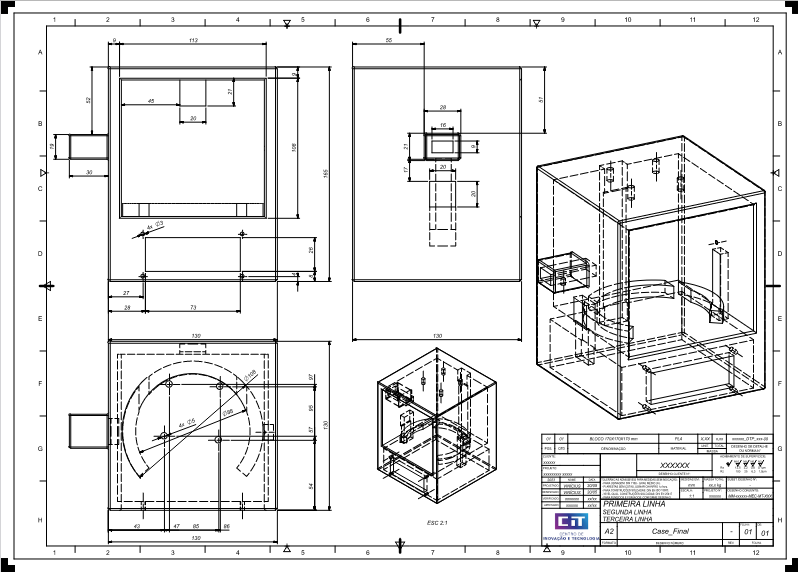
\includegraphics[width=\textwidth]{nx.png}
\caption{Projeto criado no \href{https://plm.sw.siemens.com/en-US/nx/}{NX} para impressão 3D}
\end{figure}
\begin{enumerate}
\item \href{https://www.eletrogate.com/placa-wemos-d1-esp32-wifi-bluetooth}{ESP32};
\item \href{https://www.eletrogate.com/cooler-ventoinha-radial-5015-12v}{Ventoinha de 12V};
\item \href{https://www.eletrogate.com/sensor-de-obstaculo-reflexivo-infravermelho}{Sensor infravermelho de obstáculo};
\item \href{https://www.eletrogate.com/display-lcd-16x2-com-backlight-azul}{Display LCD 16x2 com interface I2C}.
\item \href{https://www.eletrogate.com/sensor-de-umidade-e-temperatura-dht11}{Sensor de temperatura e umidade DHT22};
\end{enumerate}
\section{Código}
\begin{lstlisting}[language=C]
#include <Adafruit_Sensor.h>
#include "DHT.h"
#include <LiquidCrystal.h>
#define DHTTYPE DHT11
uint8_t DHTPin = 27;
DHT dht(DHTPin, DHTTYPE);
#define PINFAN 25
#define PINPONTH 33
#define PINSIV 26
LiquidCrystal lcd(19, 23, 18, 17, 16, 15);
#define THRESHOLD_TEMP 25.0
#define THRESHOLD_IR 1
bool isFull = false;
float temperatura;
float umidade;
void setup() {
    Serial.begin(115200);
    dht.begin();
    pinMode(PINSIV, INPUT);
    pinMode(PINFAN, OUTPUT);
    pinMode(PINPONTH, OUTPUT);
    lcd.begin(16, 2);
}
void loop() {
    temperatura = dht.readTemperature();
    umidade = dht.readHumidity();
    int irRead = digitalRead(PINSIV);
    if (temperatura >= THRESHOLD_TEMP) {
      digitalWrite(PINFAN, HIGH);
      digitalWrite(PINPONTH, HIGH);
    } else {
      digitalWrite(PINFAN, LOW);
      digitalWrite(PINPONTH, LOW);
    }
    if (irRead == THRESHOLD_IR) {
      isFull = true;
    } else {
    isFull = false;
    }
    lcd.clear();
    lcd.setCursor(0, 0);
    lcd.print("T: ");
    lcd.print(temperatura,0);
    lcd.print("C");
    lcd.print("   ");
    lcd.print("U: ");
    lcd.print(umidade,0);
    lcd.print("%");
    lcd.setCursor(0, 2);
    lcd.print("Quanti.: ");
    lcd.print(isFull ? "Cheio" : "Vazio");
    delay(2000);
}
\end{lstlisting}
O código é estruturado em torno da leitura dos sensores, processamento dessas leituras e exibição das informações no display LCD.
As bibliotecas incluídas no início do código são necessárias para a comunicação com o hardware e a operação dos sensores e da ventoinha. O código é estruturado de forma que as operações críticas são realizadas continuamente no loop principal.
A função \verb|setup()| é executada primeiro para configurar os componentes de hardware, iniciar a comunicação serial, configurar os pinos de entrada e saída e inicializar a ventoinha em um estado desligado.
A função \verb|loop()| é executada continuamente e é aqui que o sensor de temperatura e umidade (DHT22) é lido, o estado do sensor infravermelho é verificado, a ventoinha é controlada e os resultados são exibidos no display LCD.
\section{Monitoramento da Temperatura e Umidade}
A temperatura e umidade são lidas do sensor DHT22. Se a temperatura lida exceder um valor limite definido (por exemplo, 25 graus Celsius), a ventoinha é ligada para resfriar o ambiente. Caso contrário, a ventoinha é desligada.
\section{Monitoramento do Nível do Recipiente}
O nível do recipiente é monitorado através de um sensor infravermelho de obstáculo. Se o sensor infravermelho detectar a presença de um obstáculo (indicando que o recipiente está cheio), o sistema irá registrar esse estado.
\section{Exibição de Informações}
As informações de temperatura, umidade e o estado do recipiente são exibidas no display LCD 16x2. A temperatura é exibida em graus Celsius, a umidade é exibida em porcentagem e o estado do recipiente é exibido como "Cheio" ou "Vazio".
\section{Considerações Finais}
Este código é uma base para o seu projeto e pode necessitar de modificações para se adequar ao seu hardware específico e requisitos do projeto. Por exemplo, os pinos usados para conectar os componentes do hardware, os valores limite para ativação da ventoinha ou detecção de recipiente cheio, e a forma como as informações são exibidas no display podem ser personalizadas conforme necessário. Além disso, recomenda-se verificar se os componentes estão sendo alimentados corretamente de acordo com suas especificações. O ESP32 opera com 3.3V, o DHT22 e a ventoinha de 12V podem precisar de seus respectivos reguladores de tensão.
\section{Créditos}
Agradecemos os Srs. \href{https://www.linkedin.com/in/vin\%C3\%ADcius-roberto-dos-santos-03a84619a/}{Vinicius Roberto dos Santos},\href{https://www.linkedin.com/in/j\%C3\%BAlio-pires-materiais-soldagem/}{Julio Cezar de Alvarenga Pires}, Thiago Wendel Sousa Vieira, Breno Luis de Oliveira Carvalho e toda equipe do \href{https://www7.fiemg.com.br/cit}{CIT SENAI} pela colaboração no projeto.
\end{document}

